\documentclass[titlepage, 12pt]{scrartcl}

\usepackage[utf8]{inputenc}

\usepackage{amsmath,amssymb,amsthm}
\usepackage{thmtools}

\usepackage[croatian]{babel}
\usepackage{csquotes}

\usepackage[unicode]{hyperref}
\usepackage{enumitem}
\usepackage{minted}
\usepackage{graphicx}


\MakeOuterQuote{"}


\title{Modeliranje grafovske baze podataka za društvenu mrežu - \emph{Neo4j}}
\author{Karlo Basioli \and 
        Antonela Bogdanić \and 
        Ivan Krcivoj }
\date{Lipanj 2021}

\begin{document}

\maketitle

\tableofcontents

\newpage

\section{Uvod}
Tema ovog projekta je modeliranje grafovske baze podataka za društvenu mrežu koristeći \emph{Neo4j}. Zadatak podrazumijeva odabir programskog jezika za izgradnju grafičkog sučelja, osmišljavanje i implementaciju struktura podataka potrebnih za pisanje kompleksnih upita te generiranje podataka i punjenje same baze. \\
Projekt je u potpunosti izveden koristeći \emph{Python 3.9} programski jezik uz modul \emph{tkinter} za grafičko sučelje i modul \emph{neo4j} koji omogućava spajanje na bazu. \\
U sklopu projekta potrebno je osmisliti upit za predlaganje osoba sličnih po obrazovanju i znanju te upit za predlaganje osoba po samostalno osmišljenom kriteriju.

\newpage
\section{Struktura podataka}
Prvi problem projekta je razrada struktura podataka kojima će društvena mreža biti modelirana. Kao inspiracija gledane su društvene mreže kao što su \emph{Facebook}, \emph{Twitter}, \emph{Instagram}, \emph{LinkedIn} \dots \\
Ove popularne društvene mreže danas broje stotine milijuna korisnika. Unatoč brojnim razlikama u suštini imaju sličnu poantu. Njihov zadaća je povezati korisnike. Ljudi koji koriste ove mreže mogu se međusobno dodavati za prijatelje, pratiti razne grupe, razmjenjivati poruke, dijeliti fotografije i slično. \\
Aspekt koji je gotovo uvijek zajednički je upravo spajanje korisnika. To će biti fokus ovog projekta. Potrebno je osmisliti kako reprezentirati korisnika i njegove veze sa ostalim korisnicima. Također korisnici će biti podijeljeni na smisleni način po edukaciji i njihovim vještinama.

\subsection{Vrhovi}
\subsubsection{Person}
Korisnik će u bazi podataka biti reprezentiran vrhom \emph{Person} sa sljedećim svojstvima:
\begin{itemize}
\begin{samepage}
    \item \textbf{id} identifikacija korisnika
    \item \textbf{name} ime korisnika
    \item \textbf{surname} prezime korisnika
    \item \textbf{gender} spol korisnika
    \item \textbf{date\_of\_birth} datum rođenja korisnika
    \item \textbf{skills} vještine koje korisnik dobija samostalno ili učenjem na fakultetu
    \item \textbf{hobbies} hobiji korisnika
\end{samepage}
\end{itemize}
Svaki \emph{id} postavljen je prilikom generiranja koda te je postavljen kao jedistven u bazi naredbom:
%TODO vidi kako ovo popraviti
\begin{samepage}
\begin{minted}[tabsize=1,breaklines]{mysql}
CREATE CONSTRAINT personIdConstraint ON (person:Person) ASSERT person.id IS UNIQUE;
\end{minted}
\end{samepage}
Također, kombinacija (\emph{name}, \emph{surname}) je jedinstvena zbog jednostavnosti.
\\ \\
\subsubsection{College}
Kako je važno znati edukaciju korisnika u bazi podataka nalaziti će se i vrh \emph{College} koji predstavlja fakultet te ima sljedeća svojstva:
\begin{itemize}
\begin{samepage}
    \item \textbf{id} identifikacija korisnika
    \item \textbf{name} puno ime fakulteta
    \item \textbf{short\_name} skraćeno ime fakulteta
    \item \textbf{area} područje u koje spada fakultet
    \item \textbf{skills} vještine koje polaznik ovog fakulteta može steći
\end{samepage}
\end{itemize}
Slično kao kod vrha \emph{Person} svojstvo \textbf{id} je jedinstveno. \\
Važna pretpostavka ove baze je da je svaki njen korisnik pohađao fakultet. 
\subsection{Relacije}
\subsubsection{IS\_FRIEND}
Očito važna relacija u ovoj bazi podataka je relacija \emph{IS\_FRIEND}. Ova relacija uspostavlja se između dva vrha sa oznakom \emph{Person} i govori da su ta dva korisnika prijatelji u ovoj društvenoj mreži. \\
Jedini atribut je:
\begin{itemize}
\begin{samepage}
    \item \textbf{start\_date} početak prijateljstva
\end{samepage}
\end{itemize}
Veza nije usmjerena te između dva korisnika postoji najviše jedna veza. \\ \\
\begin{center}
    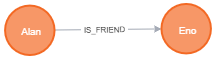
\includegraphics{slike/IS_FRIEND.png}
\end{center}

\subsubsection{SAME\_AREA}
Relacija \emph{SAME\_AREA} povezuje dva fakulteta koja spadaju u isto znanstveno područje. Ova relacija služi za skraćivanje nekih upita te dodatne atribute. \\
Veza također nije usmjerena te dva fakulteta mogu biti povezana najviše jednom ovakvom vezom. \\
U konkretnoj bazi postoje samo tri područja.
\\ \\
\begin{center}
    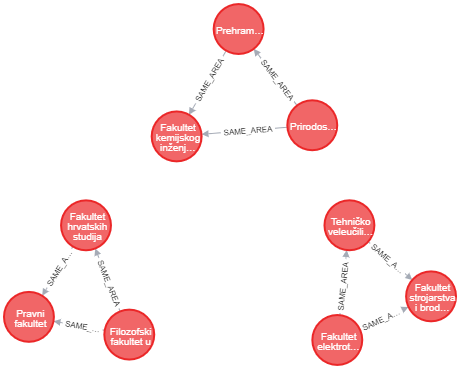
\includegraphics[scale=0.7]{slike/SAME_AREA.png}    
\end{center}

\subsubsection{ATTENDED}
Na kraju postoji i relacija \emph{ATTENDED}. Ovo je prva i jedina jednosmjerna relacija u bazi. Predstavlja vezu između korisnika i fakulteta. Ukoliko se ova dva vrha povezana bridom \emph{ATTENDED} to značni da korisnik pohađa ovaj fakultet. \\
Svojstva ove veze su:
\begin{itemize}
\begin{samepage}
    \item \textbf{enrollment\_year} godina upisa fakulteta
    \item \textbf{graduate\_year} godina završetka fakulteta
    \item \textbf{grade} prosjek ocjena dosadašnjeg studija
\end{samepage}
\end{itemize}
\begin{center}
    
\includegraphics{slike/ATTENDED.png}    
\end{center}

\newpage

\section{Generiranje podataka}
\subsection{Izvori podataka}
\subsection{Kako su podaci generirani}
\newpage

\section{Implementacija aplikacije i grafičko sučelje}
Kao što je već spomenuto za izgradnju aplikacije korišten je programski jezik \emph{Python} zbog velikog broja modula koje posjeduje i jednostavnosti korištenja tih modula. \\
Za interakciju sa bazom korišten je modul \emph{neo4j} dok se grafičko sučelje izgradilo sa modulom \emph{tkinter}.
\subsection{Modul neo4j}
Ovaj modul među nekoliko postojećih \emph{Python} modula za \emph{Neo4j} zato što je i službeno podržavan od strane \emph{Neo4j} baze podataka. \\
Za projekt je napravljena klasa \emph{Database} kao \emph{singleton} kako se ne bi nepotrebno stvarao preveliki broj različitih \emph{drivera}.

\begin{samepage}
\begin{minted}[tabsize=1,breaklines]{python}
class Database:
    __instance = None

    @staticmethod
    def get_instance(path = "database.cfg"):
        if Database.__instance == None:
            Database(path)
        return Database.__instance

    def __init__(self, path):
        if Database.__instance != None:
            raise Neo4jError("This class is a singleton!")
        else:
            #čitanje potrebnih podataka iz .cfg datoteke
            self.driver = GraphDatabase.driver(db_url, auth=(username, password))
            Database.__instance = self

    def close(self):
        self.driver.close()
\end{minted}
\end{samepage}
Prikazane su samo najosnovnije metode ove klase. \\
Instanca ove klase koristi se za slanje upita na bazu podataka. Jednostavan uzorak koji je praćen kroz cijeli projekt izgleda otprilike ovako:
\begin{samepage}
\begin{minted}[tabsize=1, breaklines]{python}
def query_database(cypher_query, args_dict, path_to_cfg):
    db = Database.get_instance(path_to_cfg)
    
    with db.driver.session() as session:
        result = session.run(cypher_query, args_dict)
    #obrada dobijenih rezultata
\end{minted}
\end{samepage}
Veliki izazov korištenja ovog modula i projekta općenito bilo je osmisliti kako puniti bazu sa generiranim podacima. Kao što je već spomenuto generirani podaci spremani su u \emph{.csv} datoteke. \\
Deklarativni jezik \emph{cypher} podržava naredbu: 
\begin{minted}{mysql}
LOAD CSV
\end{minted}
Ova naredba omogućava jednostavno učitavanje \emph{.csv} datoteka. Kako bi bilo omogućeno što jednostavnije punjenje baze za različite korisnike ove datoteke se pokretanjem \emph{Python} skripte šalju u \emph{import} direktorij čiji je \emph{path} potrebno zapisati u \emph{database.cfg} datoteku. \\
Upiti za učitavanje vrhova iz baze grade se na sljedeći način:
\begin{samepage}
\begin{minted}[tabsize=1,breaklines]{python}
def get_load_command_entity(self, file_name, header, entity):
    header = header.split(",")
    cypher = f"LOAD CSV WITH HEADERS FROM \"file:///{file_name}\" AS csv_line CREATE (p:{entity}" + "{"
    first = True

    for header_element in header:
        if first:
            cypher += add_attribute(header_element)
            first = False
        else:
            cypher += ", " + add_attribute(header_element)

    cypher += "});"

    return cypher
\end{minted}
\end{samepage}
Na ovaj način osigurano je jednostavno punjenje baze podataka za svakog korisnika pokretanjem skripti za generiranje podataka, a potom i skripte za punjenje baze.
\subsection{Tkinter}
\newpage

\section{Preporuke}
Postoje različiti načina stvaranja preporuka korisniku. Mnoge društvene mreže korisne razne alate i strojno učenje kako bi smislili najbolje moguće preporuke svojim korisnicima.
Neke od ovih društvenih mreža nerijetko se nalaze i u problemima s privatnosti zbog jako velike preciznosti njihovih preporuka.
Neki misle da ti algoritmi koriste informacije za koje korisnik nikad eksplicitno ne da dopuštenje. Takvi podaci su na primjer lokacija, članovi obitelji te su čak toliko efikasni da neki vjeruju da društvene mreže osluškuju razgovore. \\
Ovaj projekt se srećom bavi generiranim podacima te izbjegava probleme privatnosti. Cilj nije složiti model koji će učiti preferencije korisnika već iskoristiti grafovsku strukturu podataka kako bi po vezama između korisnika mogli dati što bolju preporuku po predodređenim kriterijima. \\
Slijede neke, možda očite, metode preporučivanja zaključno sa implementiranim algoritmima preporučavanja.

\subsection*{Preporuke po broju zajedničkih prijatelja}
Najjednostavniji način za dobiti broj zajedničkih prijatelja je poprilično izravan. Korisnik za preporuku dobija upravo one ljude s kojima ima najviše zajedničkih prijatelja. \\
U bazi \emph{neo4j} sljedećim upitom moguće je dobiti zajedničke prijatelje dva korisnika:
\begin{samepage}
\begin{minted}[tabsize=1,breaklines]{mysql}
MATCH (p:Person {id:72})-[i:IS_FRIEND]-(common:Person)-[j:IS_FRIEND]-
(potential_friend:Person {id: 83}) 
WHERE p.id <> potential_friend.id AND NOT ((p)-[:IS_FRIEND]-(potential_friend)) 
RETURN p, common, potential_friend,i,j;
\end{minted}
\end{samepage}
\begin{center}
    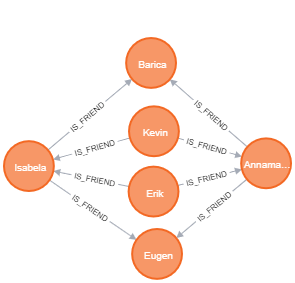
\includegraphics[scale=0.7]{slike/common_friends_query.png}
\end{center}

\subsection*{Preporuke po utjecaju}
Slično kao u prethodnom primjeru i ovdje dolazi do preporuke po zajedničkom broju prijatelja. Ipak, u ovoj metodi situacija je nešto drugačija. \\
Pretpostavimo da imamo korisnika \emph{p} i korisnika \emph{potential\_friend} koji imaju zajedničke prijatelje, ali nisu međusobno prijatelji. \\
Pretpostavimo da su njihovi zajednički prijatelji $commons = \{c_1, c_2, \dots, c_n\}$ za koje je $friends\_num(c_i)$ jednak broju prijatelja koje korisnik $c_i$ ima. \\
Što korisnik $c_i$ ima manji broj prijatelja smatran je korisnikom koji je selektivniji u izboru svojih prijatelja. Ponekad ima smisla da veću težinu donosi selektivnija osoba zato što je izglednije da ima osobnu vezu sa korisnikom. \\
Korisniku $potential\_friend$ dodjeljuje se ocjena izračunata kao suma recipročnih $friends\_num(c_i)$ gdje su $c_i$ zajednički prijatelji korisnika $p$ i korisnika $potential\_friend$. \\
Formula za izračun ocjene izgleda ovako:
\begin{equation*}
    rating(potential\_friend) = \sum_{c \in commons} \frac{1}{friends\_num(c)}
\end{equation*}
Osoba sa najvećim \emph{ratingom} biti će prva preporuka po ovom algoritmu. \\
Dobro je primjetiti da je razlomak u gornjem izrazu uvijek dobro definiran pošto svaki korisnik $c$ ima barem dva prijatelja s obzirom da je on zajednički prijatelj korisnicima $p$ i $potential\_friend$. \\
Slijedi upit kojim bi se izračunao \emph{rating} korisnika u \emph{cypheru}.

\begin{samepage}
\begin{minted}[tabsize=1,breaklines]{mysql}
MATCH (p:Person {id:72})-[:IS_FRIEND]-(common:Person)-[:IS_FRIEND]-
(potential_friend:Person {id: 83}) 
WHERE p.id <> potential_friend.id AND NOT ((p)-[:IS_FRIEND]-(potential_friend)) 
WITH common, potential_friend
MATCH (common)-[r:IS_FRIEND]-(:Person)
WITH COUNT(r) AS friends_num, common, potential_friend
RETURN SUM(1.0/friends_num) AS rating, potential_friend;
\end{minted}
\end{samepage}

\subsection*{Klasifikacijske preporuke}
Ovakav tip preporuka gleda zajednička svojstva dva korisnika i na temelju toga donosi odluku tko je kome najsličniji. \\
Za ovu bazu zajedničko svojstvo korisnika može biti fakultet koji oba korisnika pohađaju, a moguće ih je poredati po broju istih vještina koje imaju.Ovakva preporuka ima smisla zato što je logično da će se ljudi sa istog fakulteta poznavati te da je veća vjerojatnost da će se želiti sprijateljiti ako su njihove vještine iste. \\
\newpage
Primjer upita koji prikazuje sve studente na jednom fakultetu:

\begin{samepage}
\begin{minted}[tabsize=1,breaklines]{mysql}
MATCH (p:Person)-[att:ATTENDED]->(c:College {short_name: "TVZ"})
RETURN p, c, att LIMIT 10;
\end{minted}
\end{samepage}

Rezultat istog upita:
\begin{center}
    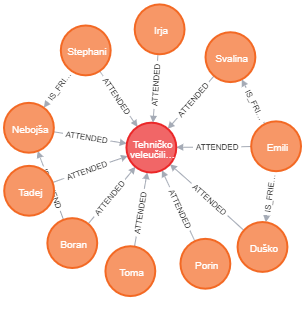
\includegraphics[scale=0.7]{slike/same_college.png}
\end{center}

Ovo su neke od metoda koje se mogu koristiti za preporuke u društvenim mrežama te su poslužile kao inspiracija za upite kojima aplikacija predlaže korisnicima njihove potencijalne prijatelje. \\
Dio projekta bio je osmisliti upite koji će predlagati prijatelje na temelju znanja i obrazovanja te za osobne preporuke.

\subsection{Poslovne preporuke}
Želja je omogućiti korisniku brzo i efikasno umrežavanje sa ljudima istih ili sličnih vještina. \\
Izglednije je da će korisnik dodati osobu sličnih vještina zbog mogućnosti suradnje. Ovo podosta zvuči kao klasifikacijska preporuka no je li moguće dodatno personalizirati preporuke na temelju postojećih informacija? \\
Podosta je očito da je korisniku važno upoznati ljude sa srodnih fakulteta. To će biti prvi filter preporuka.\\
Upit je prezentiran u koracima. \\
U idućem upitu primjetite nizove znakova nakon dolara. To su vrijednosti koje korisnik predajem prilikom slanja upita. Ako je aplikaciju  uključila osoba sa identifikacijskim brojem $14$ tada će se idući upit izvršiti sa tim identifikacijskim brojem.

\begin{samepage}
\begin{minted}[tabsize=1,breaklines]{mysql}
MATCH (p:Person {id:$id})-[:ATTENDED]->(:College)-[:SAME_AREA]-
(:College)<-[:ATTENDED]-(recommendation:Person)
WHERE p.id <> recommendation.id AND NOT((p)-[:IS_FRIEND]-(recommendation))

\end{minted}
\end{samepage}
Idući dio ovisi o korisniku. Ljudi različitog godišta imaju različite poslovne interese. \\
Mlađi ljudi će zbog srama, neiskustva i sličnog teže pristupiti  iskusnijoj osobi. Izglednije je da će mlađa osoba htjeti dodati svoje vršnjake koji imaju slična iskustva. \\
S druge strane iskusnija osoba mari manje za to i više ju zanimaju vještine korisnika. Na primjer poslodavcu može biti zanimljivo zaposliti studenta kao ulaganje u budućnost, ali može mu od interesa biti i zapošljavanje iskusnih ljudi iz njegovog područja. \\
Dakle idući filter za mlade ljude biti će razlika u godinama, što je manja izglednije je da će joj se ta osoba preporučiti dok će za starije ljude filter biti presjek istih vještina koje osoba ima. \\
Sada kada su preporuke dodatno sužene, ako je to potrebno, opet po godištu dodajemo nove filtere. \\
U ovom slučaju ćemo zamijeniti uloge. Mlađi ljudi će sada u svojem popisu preporuka imati ljude sličnog godišta pa će se te preporuke filtrirati po presjeku vještina zato što je izglednije da će mladi ljudi htjeti dodati osobu zainteresiranu za njihovo područje. \\
S druge strane starijim korisnicima filter će analogno mlađim korisnicima poredati preporuke po razlici u godinama tako da ipak za početak dobiju najiskusnije ljude iz svog područja. \\
Slijedi nastavak na prethodni komad koda sastavljen od navedena dva filtera za starije korisnike:
\begin{samepage}
\begin{minted}[tabsize=1,breaklines]{mysql}
WITH p, recommendation, size([x IN p.skills WHERE x IN recommendation.skills]) AS common_skills 
ORDER BY common_skills DESC LIMIT $first_limit
RETURN recommendation, abs(p.date_of_birth.year - recommendation.date_of_birth.year) AS birth_delta 
ORDER BY birth_delta DESC LIMIT $limit;

\end{minted}
\end{samepage}
\newpage
Rezultat sljedećeg upita za korisnicu Lori Vulin vidljiv je na grafičkom sučelju:

\begin{center}
    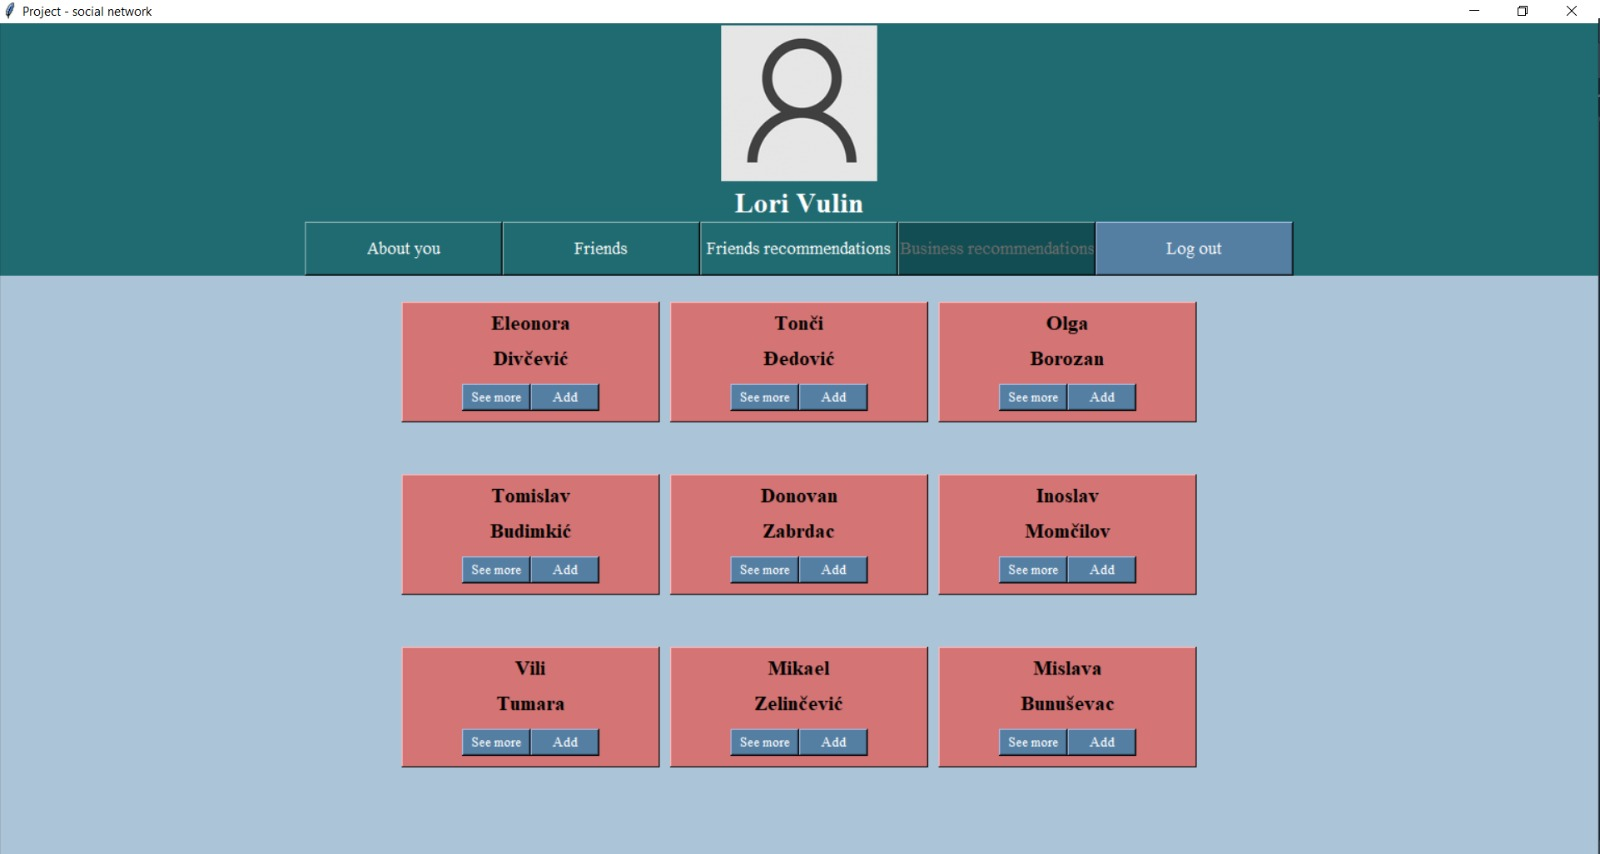
\includegraphics[scale=0.19]{slike/business.jpg}
\end{center}

\subsection{Osobne preporuke}
Slično kao poslovne preporuke osobne preporuke se odvijaju u nekoliko koraka. \\
Prvi korak je odabir osoba sa najviše zajedničkih prijatelja kako bi postojala veća vjerojatnost poznanstva.
\begin{samepage}
\begin{minted}[tabsize=1,breaklines]{mysql}
MATCH (p:Person {id:$id})-[:IS_FRIEND]-(:Person)-[:IS_FRIEND]-(recommendation:Person)
WHERE p.id <> recommendation.id AND NOT((p)-[:IS_FRIEND]-(recommendation))
WITH p, recommendation, count(recommendation) AS common_friends
ORDER BY common_friends DESC LIMIT $first_limit

\end{minted}
\end{samepage}
Ovaj puta je drugi korak za sve isti. Ljudi se češće druže sa ljudima oko svojeg godišta pa idući filter odabire najbliže ljude po godištu:
\begin{samepage}
\begin{minted}[tabsize=1,breaklines]{mysql}
WITH p, recommendation, abs(recommendation.date_of_birth.year - p.date_of_birth.year) AS birth_delta 
ORDER BY birth_delta LIMIT $second_limit

\end{minted}
\end{samepage}

Finalno potrebno je provjeriti kombatibilnost korisnika. Ovaj put osim presjeka vještina u obzir je uzet i presjek hobija. \\
Očito može biti važno da ljudi imaju iste vještine s obzirom da iz toga često proizlaze poznanstva, ali istom logikom važan je i presjek hobija. \\
Ako se dvoje ljudi bavi istom aktivnosti u slobodno vrijeme izgledno je da bi se mogli slagati ili se već poznaju. \\
Ovime se finalizira upit koji za osobne preporuke ljudima:
\begin{samepage}
\begin{minted}[tabsize=1,breaklines]{mysql}
RETURN recommendation, size([skill IN p.skills WHERE skill IN recommendation.skills]) + size([hobby IN p.hobbies WHERE hobby IN recommendation.hobbies]) AS common 
ORDER BY common DESC LIMIT $limit;

\end{minted}
\end{samepage}
\newpage
\begin{samepage}
Rezultate upita moguće je vidjeti na grafičkom sučelju:
\begin{center}
    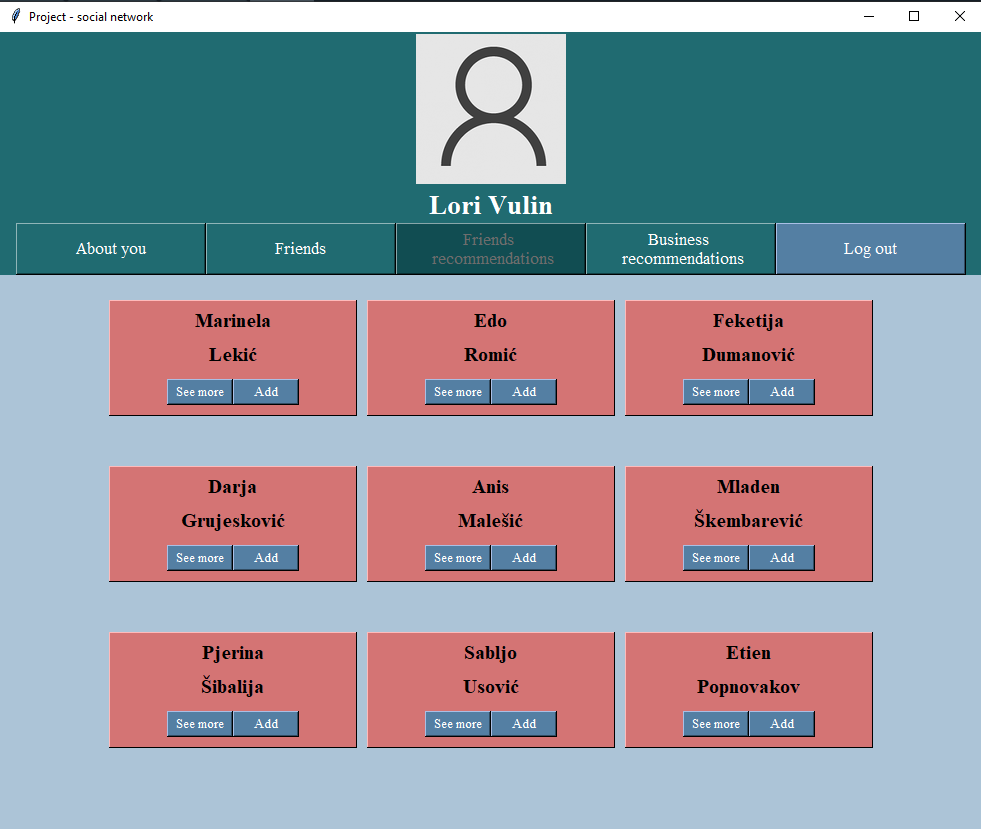
\includegraphics[scale=0.19]{slike/personal.jpg}
\end{center}
\end{samepage}

\subsection{Brzina izvršavanja upita}
Zanimljiva stvar koja je uočena prilikom stvaranja aplikacije je neovisnost trajanja upita o veličini baze. Odabrani su najsloženiji upiti, što su upravo upiti za preporučavanje prijatelja te se \emph{Pythonovom} bibliotekom \emph{time} mjerilo vrijeme izvršavanja svakog upita. \\
Napravljeno je po deset baza za svaku od veličina iz skupa $\{50, 100, 150, \dots, 1000\}$ gdje elementi skupa predstavljaju broj osoba koji se nalaze u bazi podataka. Za svaku od tih baza upit je poslan za tri nasumično odabrana korisnika te su dobijeni sljedeći rezultati.\\

\begin{center}
    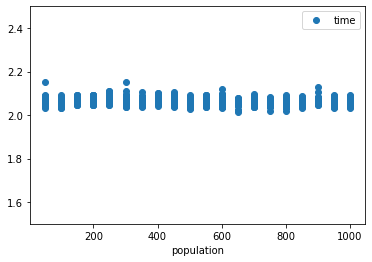
\includegraphics[scale=0.5]{slike/personal_graph.png}
    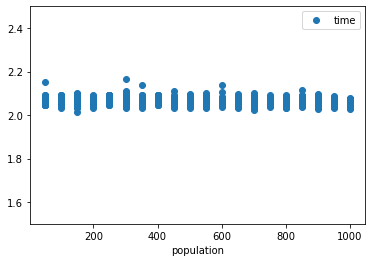
\includegraphics[scale=0.5]{slike/business_graph.png}
\end{center}


Iznenađujuće vrijeme izvršavanja upita ostaje konstantno te traje nešto više od dvije sekunde. \\
Iako na prvu ruku rezultat izgleda neočekivano razlog u tome nalazimo na naviku korištenja relacijskih baza podataka gdje bi za većinu ovakvih upita bilo potrebno raditi Kartezijev produkt tablica za što je prirodno očekivati da će rastom veličine tablice trebati puno više vremena. \\
Međutim ovdje ne dolazi do Kartezijevog produkta već se pretraživanje odvija grafovskim algoritmima što daje veliko ubrzanje 


\newpage
\section{Zaključak}

\end{document}
